\section{Emilia-Romagna Grand prix}

\subsection{Circuit Analysis}

\textbf{Circuit Name:} Autodromo Enzo e Dino Ferrari (Imola, Italy) \\
\textbf{Length:} 4.909 km - \textbf{Laps:} 63 - \textbf{Total Distance:} 309.049 km

\begin{figure}[H]
    \centering
    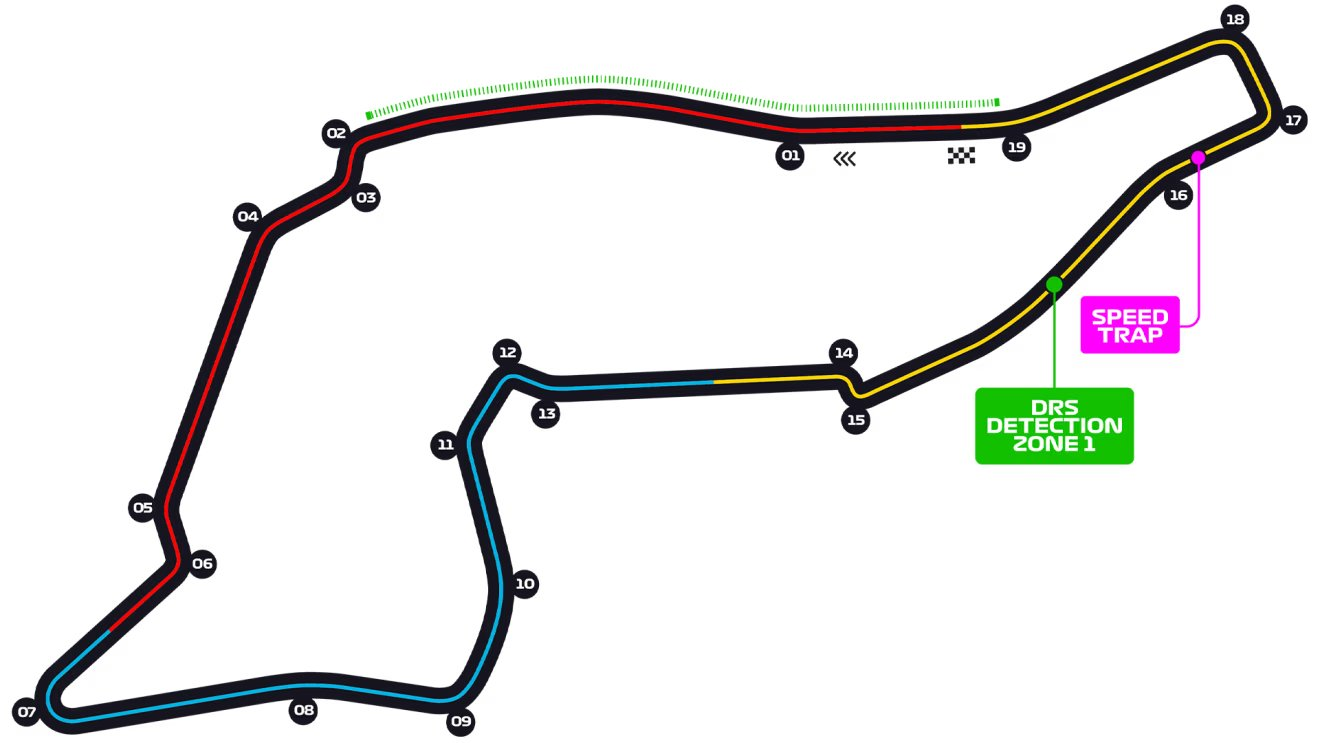
\includegraphics[width=0.75\linewidth]{images/7.Emilia_Romagna_Circuit.jpg}
\end{figure}

\begin{itemize}
    \item \textbf{Lap Record} : 1:13.609 (2020, Valtteri Bottas - Mercedes).
    
    \item \textbf{Number of Corners \& Key Features} : 19 turns (9 right, 10 left)
    
    \item \textbf{Braking Zones \& Traction} : Heavy braking at Variante Alta and Turn 1 chicane.\\
    Strong traction required exiting Rivazza onto the main straight.
    
    \item \textbf{DRS \& Overtaking} : Single DRS zone along the main straight. Overtaking possible at Turn 2 (Tamburello) after the DRS, but otherwise limited.
    
    \item \textbf{Tyre Degradation \& Strategy} : Tyre wear moderate, a one-stop Medium–Hard is the preferred strategy.\\
    Track position critical due to limited overtaking.
    
    \item \textbf{Weather \& Environment} : Spring in Emilia-Romagna brings variable conditions, risk of rain often present. Track is narrow with little runoff, making mistakes costly.
\end{itemize}

\textbf{Strategic Summary :}
Imola emphasises track position, consistency, and precision. Qualifying is vital, as overtaking is difficult. One-stop strategies are common, but Safety Cars can create opportunities.


\subsection{Race Analysis}

\textbf{Date:} 19 May 2024 — 15:00 local time 

\begin{itemize}
    \item \textbf{Qualifying Summary} : \textbf{Pole Position:} Max Verstappen (Red Bull) – 1:14.746. \\
    Grid: Norris 2nd, Leclerc 3rd, Sainz 4th.
    Oscar Piastri, who finished 2nd during the qualifications, was penalised of three grid places for impeding.
    
    \item \textbf{Race Summary} : \textbf{Winner:} Max Verstappen (Red Bull).\\
    \textbf{Podium:} 1. Verstappen - 2. Norris - 3. Leclerc.\\
    \textbf{Technical issues:} Sainz (overheating, struggled all race).\\
    Verstappen led most of the race but struggled with tyre wear late on. Norris closed the gap to 0.7s at the finish, but DRS wasn’t enough to force a pass. Leclerc consistent in P3. \\
    Sainz faded with overheating and was undercut by Piastri for P4. Mercedes steady in P6–P7. Pérez only P8, struggling in traffic.
    
    \item \textbf{Strategies} : Majority followed Medium–Hard one-stop strategy.\\
    - Norris attempted an undercut but was held in traffic, losing crucial time. \\
    - Verstappen stopped early to cover Norris.\\
    - Ferrari also on Medium–Hard but Leclerc lacked the pace to challenge McLaren.
    
    \item \textbf{Performance Trends} :\textbf{Red Bull} — Still strongest in qualifying and defending track position, but tyre wear was an issue late in stints. 
    \textbf{McLaren} — Norris showed real pace and tyre conservation, only limited by traffic and overtaking difficulty. 
    \textbf{Ferrari} — Consistent podium pace, but lacked the raw speed to pressure Red Bull and McLaren. 
    \textbf{Mercedes} — Solid points but a step behind. Russell’s fastest lap masked underlying lack of pace.
    
    \item \textbf{Championship Impact} : \textbf{Drivers:} Verstappen 161 points, Leclerc 113 (+1), Pérez 107 (-1).\\
    \textbf{Constructors:} Red Bull 268, Ferrari 212, McLaren 154, Mercedes 79.    
\end{itemize}

\textbf{Key Takeaway :}
Verstappen’s defensive driving under pressure secured victory. McLaren confirmed their rise with Norris pushing Verstappen to the limit. Ferrari solid but lacked enough speed to fight for the win at home.


\subsection{Link \& Takeaway}

\begin{itemize}
    \item Imola’s narrow layout and lack of overtaking rewarded Verstappen’s pole and strong defence.  
    \item Norris and McLaren showed they could pressure Red Bull on pure pace, but traffic in pit strategy denied them a shot at victory.
    \item Ferrari’s limitations in long-run pace were exposed on home soil, despite Leclerc’s podium. 
    \item Track position proved decisive, underlining Imola’s strategic rigidity.
\end{itemize}